\documentclass[10pt,twocolumn,letterpaper]{article}
\usepackage[pagenumbers]{cvpr}
\usepackage[T1]{fontenc}
\usepackage{microtype}
\usepackage[hidelinks]{hyperref}
\hypersetup{pdftitle={Learning a Writing Rubric from Edits: Context or Weights?}}
\raggedbottom
\hfuzz=0pt\vfuzz=0pt
\newcommand{\claim}[2]{#2}
\title{Learning a Writing Rubric from Edits: Context or Weights?}
\author{Research draft}
\begin{document}
\maketitle
\begin{abstract}
\claim{C01}{We study whether a writer can learn a hidden writing rubric from editorial revisions through context or weight adaptation. An inferred playbook and corrected-target LoRA receive a shared archive of synthetic reviews, and Qwen3-8B is evaluated on fresh tool-based writing assignments.}
\claim{C02}{At 480 review opportunities, averaging three method seeds, SFT achieves 89.1\% validity-adjusted rubric compliance versus 71.7\% for the inferred playbook, a 17.4-point difference with paired 95\% interval $[15.4,19.5]$.}
\claim{C03}{Mean valid submission is 96.2\%, within three points of the 97.9\% unadapted base, although one training seed falls below that safeguard. Only 46.1\% of SFT episodes produce a valid submission satisfying every applicable rule.}
\claim{C04}{These results establish substantial rubric adaptation for the tested recipes, while separating rule compliance from public-task validity and leaving prose quality unmeasured.}
\end{abstract}

\begin{figure*}[t]
\centering
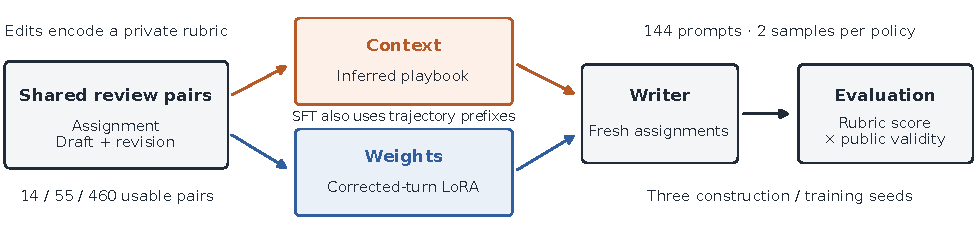
\includegraphics[width=\textwidth]{evidence/workflow.pdf}
\caption{\claim{F01}{The two learned adaptation routes share public-valid review pairs. Private rubric labels are withheld from both learners; SFT also conditions on original trajectory prefixes. Each budget starts with a fresh playbook or adapter, and evaluation uses fresh assignments.}}
\label{fig:workflow}
\end{figure*}
\section{Introduction}
\claim{C10}{We study a writer that must learn an eight-rule writing rubric from editorial revisions while satisfying public assignment constraints. The question is whether to retain what the edits teach in context or in model weights.}
\claim{C11}{When adaptation methods collect their own reviews, their comparison mixes differences in the learner with differences in the available examples. A shared review archive lets us compare the two recipes on the same corrections.}

\claim{C12}{We compare an inferred instruction playbook with corrected-target supervised fine-tuning (SFT), using a common synthetic archive and fresh assignments. SFT also sees trajectory prefixes, so the comparison shares review pairs without equalizing conditioning information or computation.}
\claim{C13}{We distinguish compliance with the private rubric, valid submission under public constraints, and performance on a separate instruction-following probe.}

\claim{C18}{Our central finding is a 17.4-point endpoint advantage for SFT in validity-adjusted rubric compliance. Lower-budget validity failures and training-seed variation qualify that gain, making task completion a separate part of the comparison rather than an assumed consequence of learning the rubric.}

\section{Related work}
\claim{C20}{Inferring preferences from edits and retrieving them later, as in CIPHER~\cite{cipher}, lets corrections influence future contexts without fine-tuning. Our fixed-archive comparison adds weight adaptation and measures public-format failures.}
\claim{C21}{Maintained playbooks provide another contextual representation: Agentic Context Engineering incrementally updates itemized instructions~\cite{ace}. We adopt delta updates, without reproducing its full reflection and curation pipeline.}

\claim{C22}{Comparisons of contextual demonstrations and fine-tuning find that their relative performance depends on data scale and task~\cite{bertsch}, motivating measurements at several budgets rather than a universal crossover claim.}
\claim{C23}{LoRA supplies low-rank weight updates~\cite{lora}; OPPU combines personal adapters with nonparametric context~\cite{oppu}. These support testing a weight-only recipe and its combination with a playbook.}
\claim{C24}{Mechanically checkable instructions in IFEval~\cite{ifeval} provide a separate spillover probe. Work on language-model evaluation motivates paired comparisons and attention to clustered questions~\cite{miller}.}

\section{Method}
\subsection{Task and writing rubric}
\claim{C32}{The writer uses JSON file operations, a format check, and submission actions to produce a 120--350-word story containing two required words; at most eight assistant tool turns are allowed.}
\claim{C33}{The public checker verifies word count and anchors, and submission requires a successful check of the current story; it does not judge plot adherence, coherence, literary quality, or the private rubric.}
\claim{C34}{Eight private checks ban ``suddenly'', ``very'', semicolons, and em dashes; require at least 90\% present finite narration verbs, an opening of at most 12 words, say-only detected dialogue tags, and restricted capitalization, using fixed regex and spaCy rules.}

\claim{C35}{Let $U$ indicate a valid submitted story and $S$ be the fraction of applicable private rules passed; the primary score is $Y=US$, assigning invalid or unsubmitted episodes zero and omitting the dialogue-tag rule when no qualifying tags occur.}
\claim{C36}{We also report $S$ conditional on validity, all-rule success $U\mathbf{1}[S=1]$, and the harder-rule score $U(r_{\mathrm{tense}}+r_{\mathrm{opening}}+r_{\mathrm{capitalization}})/3$, because several rubric rules have high baseline pass rates.}

\subsection{Learning from shared edits}
\claim{C30}{We reuse 480 earlier no-feedback Qwen3-8B review opportunities, of which 460 contain both a publicly valid writer submission and a publicly valid Inkling revision; budgets of 15, 60, and 480 opportunities yield 14, 55, and 460 usable pairs.}
\claim{C55}{The archived editor configuration supplies all eight private rules and requests minimal revisions. It asks for sentence replacements preserving meaning and required words; semantic preservation is not checked. Pair selection requires a valid draft and an archived revision recorded as successfully applied and publicly valid, without filtering for rubric-score improvement.}
\claim{C31}{The archive contains existing synthetic reviews, not human edits; the two primary learned arms use the same usable pairs at each budget.}
\claim{C41}{The no-feedback policy is unadapted Qwen3-8B; raw context uses BM25-ranked assignment matches and their before/after stories, greedily packed within 8,000 tokens.}

\claim{C42}{The playbook compiler is Inkling with temperature 0.3 and effort 0.6; it sees public assignments and before/after stories in batches of at most 15 valid pairs, proposing evidence-linked additions, replacements, or deletions to numbered instructions.}
\claim{C43}{Each budget and construction seed starts with an empty playbook; local code applies the deltas and enforces a 2,000-Qwen-token cap, with at most two validation-only repairs for malformed updates; the compiler never receives private rules, scores, or editor audit labels.}
\claim{C44}{SFT replaces the final story-modifying action with the edited story and replays the trajectory; loss covers that assistant turn only, under its actual generation prefix, averaging over supervised tokens per example.}
\claim{C45}{Adapters have rank 16 on attention, MLP, and output layers, minibatches of at most 16 examples, and at least three epochs and 30 optimizer steps; the development-selected learning rate is $4.7\times10^{-4}$ for all three review budgets.}


\begin{figure*}[t]
\centering
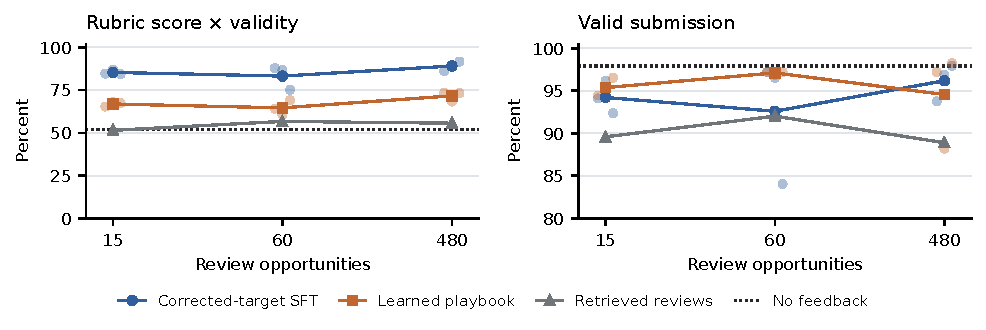
\includegraphics[width=\textwidth]{evidence/budget-comparison.pdf}
\caption{\claim{F02}{Validity-adjusted rubric score and public validity across review budgets. Large markers show means; faint points show the three method seeds, not confidence bounds. The validity axis begins at 80\%. Budgets are categorical checkpoints and connecting lines only guide the eye.}}
\label{fig:budgets}
\end{figure*}
\section{Experiments}
\subsection{Assignments and configuration}
\claim{C37}{Development uses 24 new assignments, while the sealed test set contains 144 assignments from 24 distinct places, with six assignments per place and equal numbers in familiar genres and fable/gothic.}
\claim{C38}{The generator separates development and test places, goals, and complications, rejects repeated anchor pairs and cross-split eight-word premise overlaps with the earlier prompts, and uses two stochastic samples per assignment.}

\claim{C15}{On 48 development episodes, the most valid adapter submitted 45 valid stories versus 47 for the base; none of three learning rates passed the declared base-minus-three-percentage-point validity safeguard.}
\claim{C16}{The prespecified fallback selected the highest-validity candidate, fixing its learning rate before test evaluation while retaining the failed safeguard.}
\claim{C17}{Each review budget initializes a fresh adapter from the base model; this evaluates cumulative adaptation, not sequential updates.}
\claim{C46}{We use training and compiler seeds 31, 73, and 127; generation uses the non-thinking renderer, temperature 0.7, top-p 0.8, top-k 20, and matched sampling seeds across arms.}
\claim{C53}{Schema-only compiler repairs were added after base and 15-review retrieval evaluation, before learned-policy test responses or confirmatory training; the audit preserves this amendment.}

\subsection{Comparisons and uncertainty}
\claim{C47}{The primary contrast is mean SFT minus playbook at 480 opportunities; other budgets and contrasts are exploratory, and these three checkpoints do not locate a precise review-count crossover.}
\claim{C48}{We average samples and method seeds within each assignment, then use 10,000 paired prompt-cluster bootstrap draws within familiar and fable/gothic strata for a percentile 95\% interval, with a place-cluster sensitivity interval accounting for shared locations.}
\claim{C49}{Intervals condition on the three method seeds, archive, and premise generator. We also report seed variation and flag mean validity more than three points below the base; this descriptive safeguard is not a noninferiority test.}

\claim{C50}{Follow-up controls combine SFT with its corresponding playbook, train on unedited drafts, shuffle edited targets while remapping required anchors, and supply the explicit planted rules to an unadapted privileged reference.}
\claim{C54}{After observing the verbatim-rule reference, we fixed one compact, imperative rendering that prioritizes difficult requirements and omits detector detail. This additional privileged control probes instruction presentation on the reused test set; it is exploratory and does not measure learned rubric inference.}
\claim{C51}{A separate probe uses 128 public IFEval examples selected by a fixed hash of example IDs before responses, with one response per example/policy and a 4,096-token cap; we report official strict prompt-level and instruction-level accuracy for the base, endpoint adapters, and active playbooks.}
\claim{C56}{For prompt-accuracy contrasts, we average the three method seeds within each IFEval example before contrasting with the base, then form percentile 95\% intervals from 10,000 paired example-bootstrap draws.}
\claim{C52}{Either adaptation can be disabled to restore the base policy. The public instruction subset measures active-policy spillover, with possible pretraining contamination and conflicts between the active playbook and benchmark instructions.}

\section{Results}
\subsection{Rubric learning and valid submission}
\claim{C60}{At 480 review opportunities, SFT scores 89.1\% versus 71.7\% for the playbook and 52.0\% for the unadapted base (Table~\ref{tab:endpoint}). The primary difference is $+17.4$ percentage points, with paired prompt interval $[15.4,19.5]$ and place-cluster interval $[15.2,19.6]$.}
\claim{C61}{Mean validity is 96.2\% for SFT, 94.6\% for the playbook, and 97.9\% for the base. SFT passes the descriptive three-point safeguard; its validity difference from the playbook is $+1.6$ points, interval $[-0.5,3.7]$, which does not establish a validity advantage.}

\claim{C62}{Endpoint SFT seeds score 86.3, 89.4, and 91.7\%, with 270, 279, and 282 valid submissions out of 288. Thus the mean safeguard passes despite one seed falling below it; the prompt interval does not remove this training-seed variation.}
\claim{C63}{The harder-rule score is 79.4\% versus 54.2\%, and all-rule success is 46.1\% versus 5.6\%. The advantage therefore extends beyond the easy banned-word checks, but fewer than half of SFT episodes produce a valid submission satisfying every applicable rule.}
\claim{C64}{Among valid stories, SFT passes the short-opening check in 51.4\% versus 17.1\% for the playbook; the playbook instead leads on capitalization, 100.0\% versus 96.8\%. Rubric learning remains uneven across rules.}

\claim{C65}{At 15 and 60 opportunities, the exploratory SFT-minus-playbook gaps are 18.5 and 18.6 points, but SFT validity is only 94.2\% and 92.6\%, failing the safeguard at both budgets (Figure~\ref{fig:budgets}). The observed score advantage starts at the smallest tested budget; these measurements do not locate a threshold for reliable adaptation.}
\claim{C66}{The three endpoint playbooks occupy only 63--147 tokens despite a 2,000-token allowance. None explicitly states the 12-word opener limit. This incomplete inferred rubric motivates checking the explicit-rule reference, rather than treating the learned book as the best possible contextual policy.}

\subsection{What the controls establish}
\claim{C68}{Training on unedited drafts scores 52.9\%, versus 89.1\% for corrected targets, a difference of $-36.3$ points, interval $[-38.0,-34.5]$. Extra training on drafts therefore does not reproduce the rubric gain; the content of the corrections matters for this recipe.}

\claim{C69}{Shuffled targets score 80.1\%, $9.0$ points below SFT, interval $[-11.9,-6.3]$. Yet conditional compliance (94.6\%) and all-rule success (52.4\%) exceed SFT's 92.7\% and 46.1\%, while validity falls to 84.7\%. These mixed outcomes reinforce the distinction between compliance and completion; none establishes that stories fit their assignments.}

\claim{C67}{Combining each adapter with its corresponding playbook scores 88.1\%, a $-1.0$-point difference from SFT alone, interval $[-2.6,0.6]$. Validity falls from 96.2\% to 93.9\%, difference $-2.3$ points, interval $[-4.1,-0.6]$, although all-rule success rises to 53.8\%. Thus this exploratory combination trades better all-rule success for lower public validity without a demonstrated primary-score advantage.}

\claim{C70}{Supplying the verbatim rubric yields 62.4\% $US$, with none of 274 valid stories passing the tense check. The compact reference raises $US$ to 73.2\% and valid-story tense compliance to 73.1\%, but validity falls from 95.1\% to 85.1\%; 36 of 43 invalid stories are too short. This single exploratory prompt change alters wording, order, and detector detail together. It illustrates presentation sensitivity without establishing an optimal context policy or learning from edits.}

\subsection{Instruction-following spillover}
\claim{C71}{On the unrelated IFEval subset (Table~\ref{tab:probe}), strict prompt accuracy is 83.3\% for active SFT, 79.2\% for the active playbook, and 82.8\% for the base. Paired differences from the base are $+0.5$ points, interval $[-3.6,4.7]$, and $-3.6$ points, interval $[-8.1,0.8]$, respectively. Both intervals include zero. This small public probe supplies neither a noninferiority result nor evidence of erased capabilities; the observations concern the active policies.}

\begin{table}[t]
\centering\small
\setlength{\tabcolsep}{3pt}
\begin{tabular}{@{}lrrrr@{}}
\toprule
Method & $US$ & $U$ & $S\mid U$ & All rules \\
\midrule
No feedback & 52.0 & 97.9 & 53.1 & 0.0 \\
Retrieved reviews & 55.7 & 88.9 & 62.6 & 0.0 \\
Learned playbook & 71.7 & 94.6 & 75.8 & 5.6 \\
Corrected-target SFT & 89.1 & 96.2 & 92.7 & 46.1 \\
SFT + playbook & 88.1 & 93.9 & 93.9 & 53.8 \\
Unedited-target SFT & 52.9 & 97.0 & 54.5 & 0.0 \\
Shuffled-target SFT & 80.1 & 84.7 & 94.6 & 52.4 \\
\midrule
Verbatim rubric & 62.4 & 95.1 & 65.6 & 0.0 \\
Compact rubric & 73.2 & 85.1 & 86.1 & 22.9 \\
\bottomrule
\end{tabular}

\caption{\claim{T01}{Endpoint scores (percent). Playbook, SFT, and SFT-control rows pool three seeds; other rows use one policy. Each policy has 288 episodes. $S\mid U$ conditions on validity; all-rule success requires validity. The last two rows supply privileged rubric instructions, with the compact rendering added as an exploratory follow-up.}}
\label{tab:endpoint}
\end{table}

\begin{table}[t]
\centering\small
\setlength{\tabcolsep}{4pt}
\begin{tabular}{@{}lrr@{}}
\toprule
Policy & Strict prompt & Strict instruction \\
\midrule
No adaptation & 82.8 & 89.3 \\
Active SFT adapter & 83.3 & 89.6 \\
Active playbook & 79.2 & 86.7 \\
\bottomrule
\end{tabular}

\caption{\claim{T02}{Active-policy instruction probe (percent). Every policy answers the same 128 IFEval prompts, containing 206 instruction checks, once. Adapter and playbook rows pool three seeds. Strict prompt accuracy requires all instructions in a prompt; instruction accuracy pools individual checks.}}
\label{tab:probe}
\end{table}
\section{Discussion}
\claim{C80}{This comparison concerns learning a fixed, planted writing rubric from synthetic revisions. The public checker establishes a valid submission, and the private scorer establishes compliance with its proxies; neither establishes that a story follows its plot, is coherent, or is preferable to a human reader. The shuffled-target control is especially limited by that missing semantic endpoint.}
\claim{C81}{The recipes are not compute-matched: the 15-, 60-, and 480-opportunity adapters receive 30, eight, and three epochs, respectively, corresponding to 30, 32, and 87 steps. Together with the SFT-only trajectory prefixes and development selection at one budget and seed, this prevents attributing every difference solely to where information is stored.}
\claim{C82}{The shared archive removes variation in which review pairs are available, but leaves only one editor, writer model, planted rule set, and review corpus. Three method seeds and paired evaluation strengthen this within-setting comparison without supplying evidence about human personalization, other model families, or naturally evolving preferences.}
\claim{C83}{A subsequent study could independently test semantic adherence, compare optimization exposure, and update adapters sequentially under changing preferences. Those are distinct experiments: the present cumulative adapters and active-policy instruction probe do not demonstrate a continual learner or prevention of catastrophic forgetting.}
{\small
\begin{thebibliography}{9}
\bibitem{cipher} \claim{R01}{G. Gao et al. \href{https://arxiv.org/abs/2404.15269v3}{Aligning LLM Agents by Learning Latent Preference from User Edits}. arXiv:2404.15269v3, 2024.}
\bibitem{ace} \claim{R02}{Q. Zhang et al. \href{https://arxiv.org/abs/2510.04618v3}{Agentic Context Engineering: Evolving Contexts for Self-Improving Language Models}. ICLR, 2026.}
\bibitem{bertsch} \claim{R03}{A. Bertsch et al. \href{https://arxiv.org/abs/2405.00200v2}{In-Context Learning with Long-Context Models: An In-Depth Exploration}. NAACL, 2025.}
\bibitem{lora} \claim{R04}{E. J. Hu et al. \href{https://arxiv.org/abs/2106.09685v2}{LoRA: Low-Rank Adaptation of Large Language Models}. arXiv:2106.09685v2, 2021.}
\bibitem{oppu} \claim{R05}{Z. Tan et al. \href{https://arxiv.org/abs/2402.04401v3}{Democratizing Large Language Models via Personalized Parameter-Efficient Fine-tuning}. EMNLP, 2024.}
\bibitem{ifeval} \claim{R06}{J. Zhou et al. \href{https://arxiv.org/abs/2311.07911v1}{Instruction-Following Evaluation for Large Language Models}. arXiv:2311.07911v1, 2023.}
\bibitem{miller} \claim{R07}{E. Miller. \href{https://arxiv.org/abs/2411.00640v1}{Adding Error Bars to Evals: A Statistical Approach to Language Model Evaluations}. arXiv:2411.00640v1, 2024.}
\end{thebibliography}
}
\end{document}
